\documentclass[eng]{mgr}
\usepackage{polski}
\usepackage[utf8]{inputenc}
%\usepackage{xcolor}
\usepackage[T1]{fontenc}

%pakiety do grafiki
\usepackage{graphicx}
\usepackage{psfrag} 

%Wspomaganie tabel
\usepackage{array}
\usepackage{tabularx}
\usepackage{hhline}
%Matematyka
\usepackage{amsmath}
\usepackage{amsfonts}
\usepackage{hyperref}
\usepackage{float}
%pakiet wypisujący na marginesie etykiety równań„ i rysunkóww zdefiniowanych przez \label{}, chcąc wygenerować finalną wersję dokumentu wystarczy usunąć poniższą linię
%\usepackage{showlabels}
%\newcommand{\R}{I\!\!R} %symbol liczb rzeczywistych,
%\newtheorem{theorem}{Twierdzenie}[section] %nowe otoczenie do składania twierdzenia
\usepackage{subcaption}
\usepackage{fancyref}
\title{Zastosowanie sztucznych sieci neuronowych do predykcji wyników meczów tenisa ziemnego}
\engtitle{Artificial neural networks for predicting results of tennis matches}
\author{Szymon Płaneta}
\supervisor{dr inż. Andrzej Rusiecki} 
\field{Automatyka i Robotyka (AIR)}
\specialisation{Technologie Informacyjne \\ w Systemach Automatyki (ART)}

\begin{document}
\maketitle
\tableofcontents

\chapter{Streszczenie}


\chapter{Wstęp}

\section{Tenis}
\label{Sec:Tenis}
Tenis ziemny to jedna z najbardziej popularnych dyscyplin sportowych na świecie. Mecze rozgrywane są pojedynczo (singiel), w dwuosobowych zespołach jednej płci (debel) lub obu płci (mikst). Gra w tenisa w formie jaką mamy dzisiaj wywodzi się z Birmingham w Anglii. Początki tego sportu datowane są na lata 60. XIX wieku. Najstarszy turniej na świecie, Wimbledon, pierwszy raz odbył się w roku 1877, a w latach 1896-1924 tenis był dyscypliną olimpijską. Na listę olimpiady został ponownie wpisany w roku 1988.\cite{tenis01}

W meczu tenisa może wziąć udział każdy, kto jest w stanie trzymać rakietę. Dzięki temu ilość graczy rekreacyjnych można liczyć w milionach. Tenis jest sportem widowiskowym, dlatego zmagania profesjonalistów dostarczają wielu wrażeń i gromadzą liczną widownię. Najbardziej prestiżowymi turniejami w sezonie są cztery turnieje wielkoszlemowe: Australian Open, French Open (znany również jako Roland Garros), Wimbledon oraz US Open. Kolejną rangą turniejów w tenisie męskim są turnieje z cyklu ATP World Tour: ATP World Tour Masters 1000 (cykl dziewięciu turniejów), ATP World Tour 500 i ATP World Tour 250.\cite{tenis02}

\begin{table}[H]
\centering
\caption{Turnieje wielkoszlemowe\cite{tenis02}}
\label{Tab:Slam}
\begin{tabular}{|l|l|l|l|}
\hline
\textbf{Data}       & \textbf{Nazwa turnieju}     & \textbf{Miejsce rozgrywek} & \textbf{Nawierzchnia} \\ \hline
Styczeń - Luty      & Australian Open             & Melbourne                  & Twarda                \\ \hline
Maj - Czerwiec      & French Open  				  & Paryż                      & Ziemna                \\ \hline
Czerwiec - Lipiec   & Wimbledon                   & Londyn                     & Trawiasta             \\ \hline
Sierpień - Wrzesień & US Open                     & Nowy Jork                  & Twarda                \\ \hline
\end{tabular}
\end{table}

Ogromna liczba widzów przyciąga inwestorów, przez co dyscyplina stale się rozwija. Na przestrzeni lat ewoluowała zarówno sama dyscyplina, jak i wykorzystywany w niej sprzęt czy wyspecjalizowane metody treningowe. Zauważalny jest również bezpośredni wpływ rozwoju technologii, czego przykładem jest system Hawk-Eye pozwalający na rozstrzyganie kontrowersyjnych punktów dzięki analizie obrazu z kamer i sygnału z czujników.



\section{Uczenie maszynowe}
\label{Sec:Machine}
Uczenie maszynowe to dynamicznie rozwijająca się dziedzina nauki. Polega na takim zaprogramowaniu maszyny, aby podać jedynie algorytm, dzięki któremu będzie ona w stanie nauczyć się rozwiązywać zadany problem na podstawie pewnych danych. Nie jest implementowany algorytm bezpośrednio rozwiązujący problem. 

Przykładowe zastosowania uczenia maszynowego:
\begin{itemize}
\item Rozpoznawanie mowy
\item Aproksymacje funkcji
\item Prognozowanie trendów finansowych
\item Systemy rekomendacyjne
\item Rozpoznawanie pisma
\item Sterowanie pojazdami
\item Diagnostyka medyczna
\end{itemize}

Istnieje wiele metod uczenia maszynowego, każda z nich posiada swoje wady i zalety. Różne metody znajdują zastosowania w rozwiązywaniu różnych problemów. Niektóre ze znanych metod uczenia maszynowego to maszyna wektorów uczących, sieć bayesowska czy sieci neuronowe. 

\section{Cel projektu}
\label{Sec:Goal}
Celem projektu było stworzenie sieci neuronowej, która przewidywać będzie zwycięzcę meczu tenisa ziemnego mężczyzn (ATP World Tour) na podstawie danych statystycznych dostępnych przed meczem. Zamierzano osiągnąć możliwie najlepsze wyniki, poprzez doświadczalne określenie wpływu architektury sieci oraz rodzaju danych wejściowych na jakość osiąganych rezultatów. Predykcje najlepiej spisującego się modelu będą publikowane na portalu społecznościowym Twitter.

\section{Motywacja}
\label{Sec:Motiv}
Powodem wyboru tematu była chęć zastosowania uczenia maszynowego w sporcie, gdzie analiza wielkiej ilości danych statystycznych zaczyna odgrywać coraz większą rolę. Bardzo prawdopodobnym jest, że w niedalekiej przyszłości czołowi zawodnicy wielu dyscyplin sportowych polegać będą właśnie na analizie danych. Znajdowanie słabych punktów przeciwnika oraz dobór odpowiedniej taktyki w starciu z nim, wybór optymalnego planu treningowego, pomoc w podejmowaniu decyzji o transferach czy tytułowa predykcja wyników meczów to tylko kilka z możliwych zastosowań.  Powstawały już prace o podobnej tematyce, jednak takie wykorzystanie uczenia maszynowego nadal nie jest jednym ze sztandarowych zastosowań. Z punktu widzenia kibica tenisa ziemnego, predykcja wyników meczów to bardzo atrakcyjny temat, a zainteresowanie tematyką uczenia maszynowego i chęć rozwoju w tym kierunku ostatecznie zadecydowały o wyborze tematu projektu.


\chapter{Sieci neuronowe}
\section{Wprowadzenie}
\label{Sec:ThIntro}

\section{Neuron sigmoidalny}
\label{Sec:ThSig}

\section{Struktura wielowarstwowej sieci perceptronowej}
\label{Sec:ThMLP}

\section{Propagacja wsteczna}
\label{Sec:ThBackprop}

\section{Algorytm największego spadku gradientu}
\label{Sec:ThGrad}

\chapter{Przygotowanie danych statystycznych}
Posiadanie odpowiedniej ilości należycie przygotowanych danych to warunek niezbędny do przeprowadzenia procesu uczenia sztucznej sieci neuronowej, a w rezultacie powodzenia całego eksperymentu. Zgromadzenie i odpowiednie przetworzenie danych jest często najbardziej skomplikowaną i najbardziej czasochłonną częścią całego projektu. 

W trakcie poszukiwania i przygotowywania danych można napotkać wiele problemów:
\begin{itemize}
\item Brak dostępnych danych lub ich zbyt mała liczba
\item Dane nieaktualne
\item Różne formaty/postacie danych, konieczność ujednolicenia
\item Dane niskiej jakości, wybrakowane lub zniekształcone
\end{itemize}

Jakość danych ma znaczny wpływ na jakość wyników analizy, dlatego cały proces przygotowania danych powinien zostać przeprowadzony ze szczególną starannością. Przygotowanie danych może składać się z kilku zadań: wyboru odpowiednich danych, integracji danych pochodzących z różnych źródeł, transformacji danych do pożądanego formatu, odrzucenia nieistotnych/zniekształconych danych. Etap ten jest tak istotny, że w zadaniach analizy danych może zajmować nawet 50-70\% czasu trwania całego projektu.\cite{satt01}

\section{Baza danych}
\label{Sec:DataBase}
Istnieje wiele serwisów internetowych zajmujących się kolekcjonowaniem statystyk tenisa ziemnego. Korzystanie z takich danych nie jest jednak wygodne z perspektywy programisty - serwisy zazwyczaj nie udostępniają publicznego interfejsu, więc pobieranie danych wiązałoby się z wydobywaniem ich bezpośrednio ze stron WWW (ang. \textit{web scraping}). Mogłoby to w wielu przypadkach naruszać również warunki korzystania z tych serwisów.

Poszukując odpowiedniego zbioru danych można trafić na bazy meczów w formacie CSV (ang. \textit{comma-separated values}, wartości rozdzielone przecinkiem). Są one często dystrybuowane na licencjach otwartych, pozwalających na dowolne ich wykorzystywanie. Format CSV jest atrakcyjny dla programisty, bardzo wygodny w użyciu. Niestety dane w takich bazach bywają wybrakowane lub uszkodzone. Początkowo próbowano wykorzystać jedną z takich baz\footnote{Darmowa baza danych rozpowszechniana na licencji \textit{Creative Commons Attribution-NonCommercial-ShareAlike 4.0 International License}, dostępna pod adresem: \url{https://github.com/JeffSackmann/tennis_atp}}, jednak napotkano pewne problemy. Baza nie była aktualizowana od lutego 2016 roku, a pewne dane były uszkodzone - numery identyfikacyjne graczy niekiedy się powtarzały. Uniemożliwiło to wykorzystanie jej w projekcie.

Kolejną możliwością jest skorzystanie z aplikacji desktopowej. Nie ma ich wiele, większość takich aplikacji nie jest już wspierana. Jednym z ciągle utrzymywanych programów, który wykorzystano w niniejszej pracy jest \textit{OnCourt}. Jego baza danych jest codziennie aktualizowana. Sam program umożliwia przeglądanie wielu statystyk - wszystkie mecze wybranego zawodnika, gry na danej nawierzchni czy w wybranych turniejach, obecna i historyczne pozycje w rankingu, stosunek head-to-head\footnote{Bezpośrednie konfrontacje pomiędzy dwoma wybranymi zawodnikami.} i wiele innych. Baza danych i ilość możliwości jest naprawdę ogromna, jednak wszystko to dostępne jest z poziomu graficznego interfejsu użytkownika, co znacznie utrudnia wygodne korzystanie z tego rozwiązania. Po nawiązaniu kontaktu z firmą KAN-soft, producentem oprogramowania \textit{OnCourt}, otrzymano hasło do lokalnej bazy danych pobieranej przez program, co umożliwiło wysyłanie własnych zapytań do bazy danych.
\begin{figure}
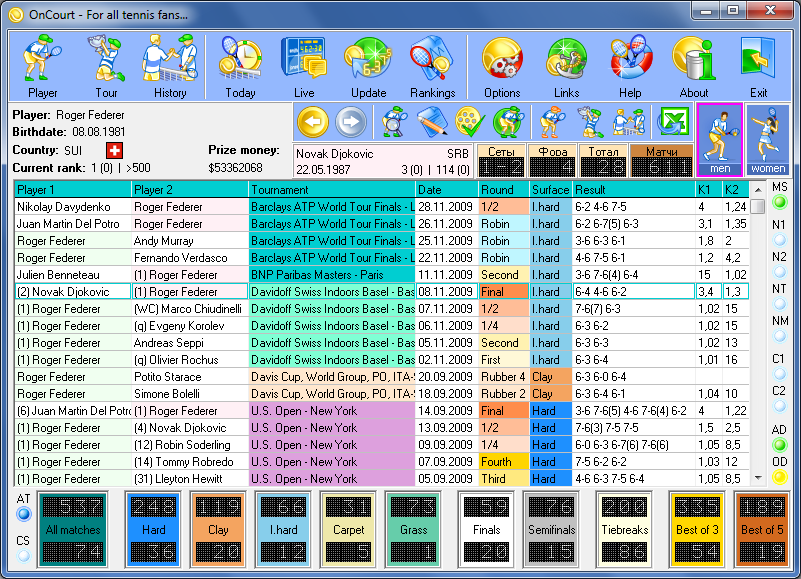
\includegraphics[width=\textwidth]{oncourt1.png}
\caption{Program OnCourt \\ (źródło: http://www.oncourt.info/)}
\label{fig:oncourt1}
\end{figure}

\section{Zastosowane technologie}
\label{Sec:DataTech}
Moduł odpowiadający za pobieranie danych z bazy, a następnie ich przetworzenie został zaimplementowany w języku Python. Python to wysokopoziomowy język skryptowy, który charakteryzuje się rozbudowanym zestawem wbudowanych bibliotek, oraz łatwością instalacji i mnogością modułów zewnętrznych.
Baza danych programu \textit{OnCourt} jest zapisywana z rozszerzeniem \textit{.mdb} - plik bazodanowy programu Microsoft Access. Do połączenia z bazą danych wykorzystano zewnętrzny moduł \textit{pyodbc}. Moduł ten pozwala na połączenie z bazami danych ODBC\footnote{Open DataBase Connectivity - interfejs umożliwiający aplikacjom dostęp do danych w bazie}. Aby było możliwe połączenie z bazą Microsoft Access, należy posiadać zainstalowane sterowniki \textit{Microsoft Access Driver (*.mdb, *.accdb)}, które dostępne są tylko dla systemu operacyjnego Windows. Po odpowiednim podłączeniu do bazy danych można wykonywać dowolne zapytania w języku SQL, a wyniki otrzymywać i przetwarzać w swoim programie.

\section{Wykorzystane statystyki}
\label{Sec:DataUsed}
Dane statystyczne wykorzystane do predykcji wyniku muszą odpowiadać danym, którymi dysponowano przed rozegraniem meczu. 
Przykładowo, aby dokonać predykcji zwycięzcy meczu między zawodnikiem A i zawodnikiem B odbywającym się w dniu 25.04.2013, należy pobrać stan z tego dnia przed rozegraniem meczu. W projekcie nie uwzględniono sytuacji, w której zawodnik może rozegrać więcej niż jeden mecz w ciągu jednego dnia, gdyż sytuacja taka ma miejsce niezwykle rzadko. Dane pobierane są na dzień poprzedzający rozegranie meczu. Wszystkie dane zostały znormalizowane i końcowe wartości używane w procesie przewidywania mają wartość z przedziału $\langle 0, 1\rangle$. 

Poniżej przedstawiono wszystkie dane statystyczne wykorzystane w projekcie, ich oznaczenia używane w dalszej części pracy, oraz krótkie uzasadnienie wyboru i sposób ich uzyskiwania:
\begin{enumerate}
\item R - Ranking zawodnika.

$R = \frac{Ranking\ zawodnika}{900}$

W przypadku braku danych: $R = 1$

Uzasadnienie: ogólna dyspozycja zawodnika w obecnym sezonie.

\item WRS - Stosunek wygranych meczów do wszystkich meczów rozegranych przez zawodnika w bieżącym sezonie.

$WRS = \frac{Wygrane\ mecze\ zawodnika\ w\ obecnym\ sezonie}{Wszystkie\ mecze\ zawodnika\ w\ obecnym\ sezonie}$

W przypadku braku danych: $WRS = 0.4$

Uzasadnienie: ogólna dyspozycja zawodnika w obecnym sezonie.

\item WR2M - Stosunek wygranych meczów do wszystkich meczów rozegranych przez zawodnika w ciągu ostatnich dwóch miesięcy.

$WR2M = \frac{Wygrane\ mecze\ zawodnika\ ostatnie\ 2\ mies.}{Wszystkie\ mecze\ zawodnika\ ostatnie\ 2\ mies.}$

W przypadku braku danych: $WR2M = 0.4$

Uzasadnienie: dyspozycja zawodnika w ciągu ostatnich dwóch miesięcy.

\item WRCT - Stosunek wygranych meczów do wszystkich meczów rozegranych przez zawodnika na korcie danego typu.

$WRCT = \frac{Wygrane\ mecze\ zawodnika\ na\ kortach\ danego\ typu}{Wszystkie\ mecze\ zawodnika\ na\ kortach\ danego\ typu}$

W przypadku braku danych: $WRCT = 0.4$

Uzasadnienie: rodzaj nawierzchni, na której rozgrywany będzie mecz ma ogromne znaczenie w tenisie. Niektórzy zawodnicy radzą sobie zdecydowanie lepiej na jednej z nawierzchni. 

\item WRTT - Stosunek wygranych meczów do wszystkich meczów rozegranych przez zawodnika w danym cyklu turniejów.

$WRTT = \frac{Wygrane\ mecze\ zawodnika\ w\ danym\ cyklu\ turniejow}{Wygrane\ mecze\ zawodnika\ w\ danym\ cyklu\ turniejow}$

W przypadku braku danych: $WRTT = 0.4$

Uzasadnienie: zdarza się, że zawodnik notuje wyjątkowo dobre lub wyjątkowo słabe występy w konkretnym cyklu turniejów.

\item H2H - Stosunek head-to-head między dwoma zawodnikami.

$H2H = \frac{Wygrane\ mecze\ zawodnika\ w\ starciu\ z\ danym\ przeciwnikiem}{Wszystkie\ mecze\ zawodnika\ w\ starciu\ z\ danym\ przeciwnikiem}$

W przypadku braku danych: $H2H = 0.5$

H2H obliczane jest tylko dla jednego z graczy występujących w meczu. Stosunek H2H dla drugiego z graczy (H2HB) w oczywisty sposób wynika z wartości H2H i wynosi $H2HB = 1 - H2H$. Z tego powodu parametr H2HB nie jest wykorzystywany.

Uzasadnienie: czasami styl gry jednego zawodnika nie odpowiada innemu zawodnikowi i jeden z nich wygrywa zdecydowaną większość spotkań.

\end{enumerate}

\chapter{Implementacja sieci neuronowej}
\section{Uniwersalny moduł MLP}
\label{Sec:MLPMod}

Celem było zaimplementowanie uniwersalnego modułu MLP (MultiLayer Perceptron - perceptron wielowarstwowy), którego będzie można dowolnie dostosowywać w zależności od potrzeb. Dotyczy to w szczególności architektury sieci (ilości wejść, ilości neuronów w warstwach ukrytych, ilości neuronów wyjściowych) oraz wykorzystywanych funkcji aktywacji, funkcji kosztów czy hiperparametrów (współczynnik uczenia, współczynnik momentu).

\section{Zastosowane technologie}
\label{Sec:MLPTech}
Moduł MLP zaimplementowano wykorzystując język Python. Do wykonywania obliczeń macierzowych użyto zewnętrznej biblioteki NumPy. NumPy to pakiet wykorzystywany do wykonywania obliczeń naukowych, a w szczególności do szybkiego przetwarzania \\ N-wymiarowych tablic. Umożliwia wykonywanie obliczeń specyficznych dla macierzy oraz łatwe wykonywanie działań element po elemencie.


\section{Struktura programu}
\label{Sec:MLPStruct}
Moduł MLP składa się z jednej klasy reprezentującej całą sieć neuronową - MLP. Zdecydowano o takiej konstrukcji, ponieważ wagi sieci przechowywane są w tablicach numpy.ndarray. Przejście sygnału przez sieć sprowadza się do wykonywania odpowiednich działań na macierzach. Utworzenie oddzielnej klasy odpowiadającej za Neuron i stworzenie sieci z obiektów klasy Neuron, skutkowałoby koniecznością wywoływania odpowiednich funkcji klasy Neuron dla każdego obiektu. Znacznie spowolniłoby to działanie całego programu. Diagram UML klasy MLP przedstawiono na rysunku \ref{fig:mlp01}.

\begin{figure}
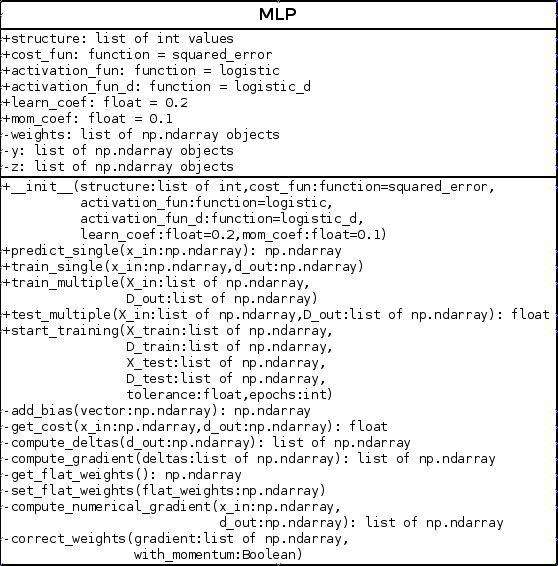
\includegraphics[width=\textwidth]{mlp01.png}
\caption{Diagram UML klasy MLP}
\label{fig:mlp01}
\end{figure}

\pagebreak

\section{Interfejs programisty}
\label{Sec:MLPAPI}

Aby skorzystać z klasy MLP wystarczy znajomość jedynie kilku metod. Proces korzystania z modułu MLP można podzielić na trzy etapy:
\begin{enumerate}
\item Stworzenie sieci o wybranej architekturze

Do stworzenia sieci o wybranej architekturze należy wykorzystać konstruktor klasy MLP. Jedynym niezbędnym parametrem jest pożądana struktura sieci, podawana w formie listy całkowitych liczb dodatnich, np. $[2, 3, 1]$ - sieć o dwóch wejściach, 3 neuronach w warstwie ukrytej i jednym neuronie wyjściowym. Pozostałe, opcjonalne parametry wraz z wartościami domyślnymi:

\begin{itemize}
\item cost\_fun (funkcja) - funkcja kosztu służąca do obliczenia wartości błędu. Domyślnie jest to błąd kwadratowy przemnożony przez 0.5.
\item activation\_fun (funkcja) - funkcja aktywacji. Domyślnie funkcja logistyczna - sigmoidalna funkcja unipolarna.
\item activation\_fun\_d (funkcja) - pochodna funkcji aktywacji. Domyślnie pochodna unipolarnej funkcji sigmoidalnej.
\item learn\_coef (float) - współczynnik uczenia. Wartość domyślna: 0.2.
\item mom\_coef (float) - współczynnik momentu. Wartość domyślna: 0.1
\end{itemize}

\item Przeprowadzenie procesu uczenia

Gdy obiekt klasy MLP jest już stworzony, można rozpocząć proces uczenia sieci. Ogranicza się to do wywołania metody start\_training. Niezbędnymi parametrami są zbiory danych: X\_train (wejściowe dane uczące), Y\_train (pożądane wyjścia odpowiadające danym podanym jako argument X\_train), X\_test (wejściowe dane testowe), Y\_test (pożądane wyjścia odpowiadające danym podanym jako argument X\_train). Opcjonalne parametry to epochs (maksymalna liczba epok\footnote{Epoka w procesie uczenia sieci neuronowych to przetworzenie całego ciągu danych uczących.}) i tolerance (gdy średni błąd spadnie poniżej tej wartości nastąpi zakończenie procesu uczenia).

\item Wykorzystywanie nauczonej sieci
W celu otrzymania odpowiedzi sieci na wektor danych wejściowych należy trzeba posłużyć się metodą predict\_single, jako argument podając jeden wektor danych wejściowych. Zwrócony zostanie wektor wyjściowy wygenerowany przez sieć.
\end{enumerate}

\pagebreak

Przykładowe zastosowanie modułu MLP do rozwiązania problemu XOR:
\begin{verbatim}
# Inicjalizacja danych wejściowych i wyjściowych
in = np.array(([1, 1], [1, 0], [0, 1], [0, 0]), dtype=float)
out = np.array(([0], [1], [1], [0]), dtype=float)

# Utworzenie sieci o strukturze: 2 wejścia, 3 neurony w warstwie 
# ukrytej, 1 neuron wyjściowy. Pozostałe parametry domyślne.
net = MLP([2, 3, 1])

# Rozpoczęcie treningu dla danych problemu XOR. Dane treningowe 
# identyczne jak dane testowe. Liczba epok 10000, gdy wartość
# błędu spadnie poniżej 0.001, nastąpi zakończenie procesu uczenia.
net.start_training(in, out, in, out, epochs=10000, tolerance=0.001)

# Wykorzystanie nauczonej sieci do predykcji
for x in in:
    net.predict_single(x)
\end{verbatim}



\chapter{Przeprowadzone doświadczenia}
\section{Porównanie wyników dla różnych architektur sieci}
\label{Sec:VsArch}

1 warstwa ukryta, rozne ilosci neuronow (powiedzmy 3 - bardzo malo (2-3), srednio (10-12), duzo (20-30), mega duzo(100)
2 wartswy ukryte

\section{Porównanie wyników dla różnych wektorów danych wejściowych}
\label{Sec:VsXIn}
rozne dane wejsciowe
- to co teraz
- jakies okrojone
+ laczna liczba rozegranych gemow w ciagu ostatnich kilku dni
+ ?????


\section{Porównanie z innymi strategiami}
\label{Sec:VsStrat}
- losowo 50\%
- zawsze ziomek wyzej w rankingu
- nizszy kurs na buku (?)
- cos jeszcze moze

\chapter{Program publikujący przewidywania sieci neuronowej na portalu społecznościowym}

\section{Zastosowane technologie}
\label{Sec:BotTech}

\section{Predykcje przedmeczowe}
\label{Sec:PredykcjePrzed}

\section{Predykcje w trakcie meczu}
\label{Sec:PredykcjeLive}

\chapter{Podsumowanie}

\bibliography{./bibliography}
\bibliographystyle{plain}

\listoffigures
\listoftables

\end{document}